\documentclass[tikz]{standalone}
\usepackage{times}
\usepackage{amsmath}
\usepackage{txfonts}
\usepackage[utf8]{inputenc}
\usepackage{graphics}
\usepackage{pgfplots}
\usetikzlibrary{arrows,intersections,math}
\usetikzlibrary{patterns}
\usetikzlibrary{pgfplots.fillbetween}
\usepackage{ifthen}
\begin{document}
	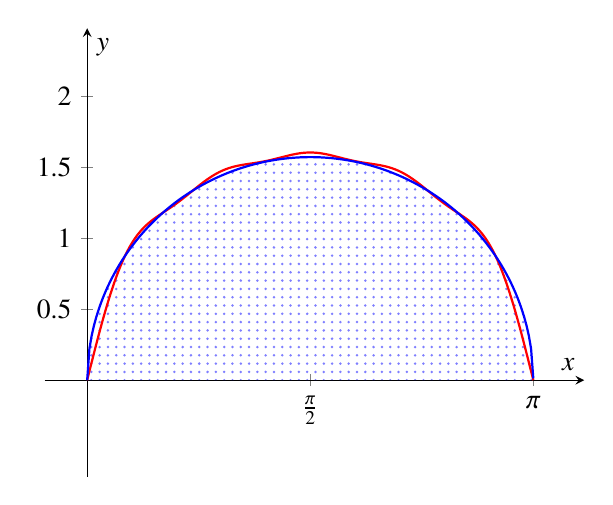
\begin{tikzpicture}
		\begin{axis}[
			axis lines=middle,
			xlabel=$x$,
			ylabel=$y$,
			xmin=-0.3, xmax=3.5,
			ymin=-0.6, ymax=2.4, 
			xtick={0, 1.5708, 3.14159},
			ytick={0.5, 1, 1.5, 2}, 
			xticklabels={0, $\frac{\pi}{2}$, $\pi$},
			axis equal=true, 
			every axis plot/.append style={thick}
			]
			\addplot[
			domain=0:3.14159,
			samples=200,
			red
			] 
			{1.7956133389*sin(deg(x)) + 0.28393414605*sin(deg(3*x)) + 0.117828104002*sin(deg(5*x)) + 0.0625789829*sin(deg(7*x)) + 0.036466961219*sin(deg(9*x))};
			
			\addplot[name path=F, domain=0:3.14159, samples=200, blue]
			{sqrt(1.5708^2-(x-1.5708)^2)};
			
			\path[name path=axis] (axis cs:0,0) -- (axis cs:3.14159,0);
			
			\addplot [
			thick,
			color=blue,
			fill=blue, 
			fill opacity=0.5,
			pattern=dots,
			pattern color=blue
			]
			fill between[
			of=F and axis,
			soft clip={domain=0:3.14159},
			split, 
			];
		\end{axis}
	\end{tikzpicture}
\end{document}